\documentclass[]{article}
\usepackage{xcolor}
\usepackage{listings}
\usepackage{showexpl}
\usepackage{graphicx}
\usepackage[bahasai]{babel}
\lstset{language=C++,
	 numbers=left,
		stepnumber=1,
	numberstyle=\ttfamily,
	basicstyle=\ttfamily,
	keywordstyle=\color{blue}\ttfamily,
	stringstyle=\color{red}\ttfamily,
	commentstyle=\color{gray}\ttfamily,
	morecomment=[l][\color{magenta}]{\#},
    breaklines=true,
    %postbreak=\mbox{\textcolor{red}{$\hookrightarrow$}\space}
}


%opening
\title{Evaluasi Tengah Semester}
\author{Akhmad Thoriq Afif NRP 5024201028}

\begin{document}
\maketitle
\section{Listing Program}
Berikut ini merupakan source code dari program implementasi array pada struktur kota, queue, dan stack. Program ini ditulis menggunakan bahasa C++
\lstinputlisting[label={kodingan},caption={Operasi dasar Dalam Array}, language={C++}]{ets.cpp}
\begin{figure}[htp]
    \centering
    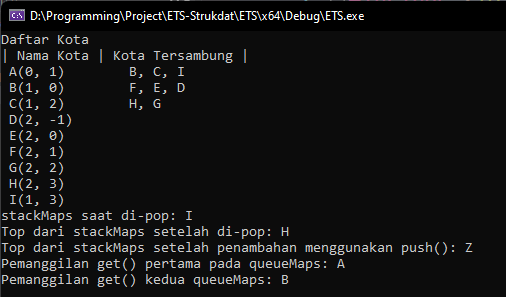
\includegraphics[width=12cm]{output.png}
    \caption{Output Program}
    \label{fig:galaxy}
\end{figure}
\begin{figure}[htp]
    \centering
    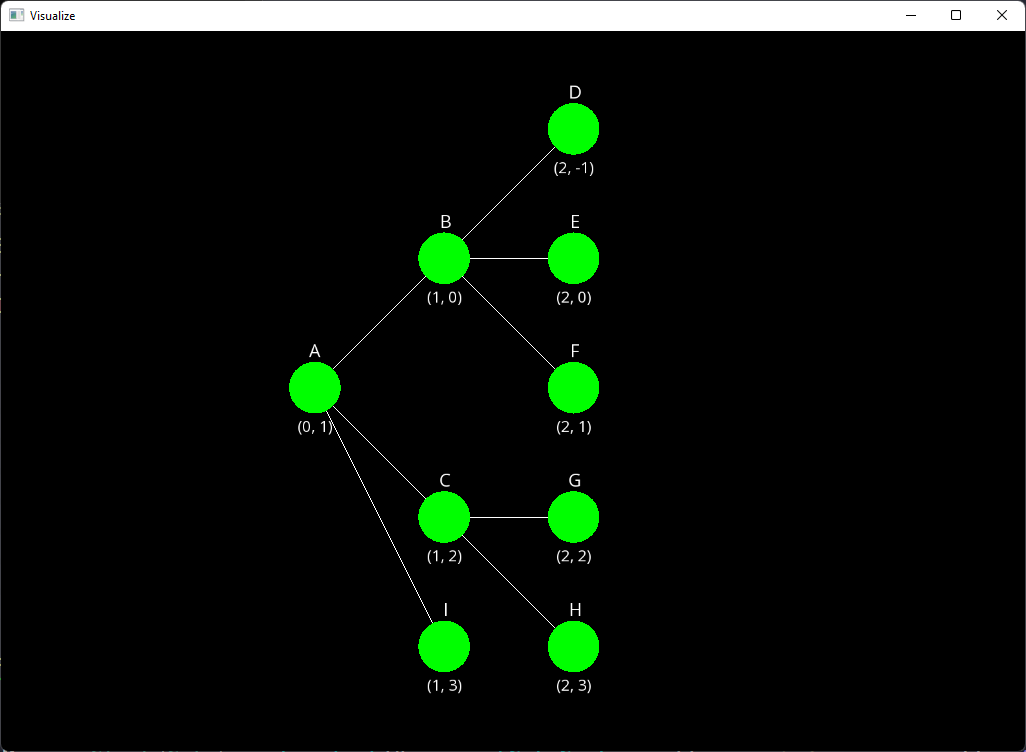
\includegraphics[width=12cm]{output-viz.png}
    \caption{Visualisasi hubungan kota menggunakan library SFML}
    \label{fig:Visualisasi}
\end{figure}
\pagebreak
\section{Desain Struktur Data}
\par
Pada program ini, terdapat beberapa class dan struct. Antara lain, Class Maps, City, Queue, dan Stack.
\subsection{Class Maps dan City}
\par
Pada class ini terdapat member class berupa array bernama mCityContainer yang berfungsi untuk menyimpan pointer dari objek City. Di bawah ini merupakan
ilustrasi dari array mCityContainer.
\begin{figure}[htp]
    \centering
    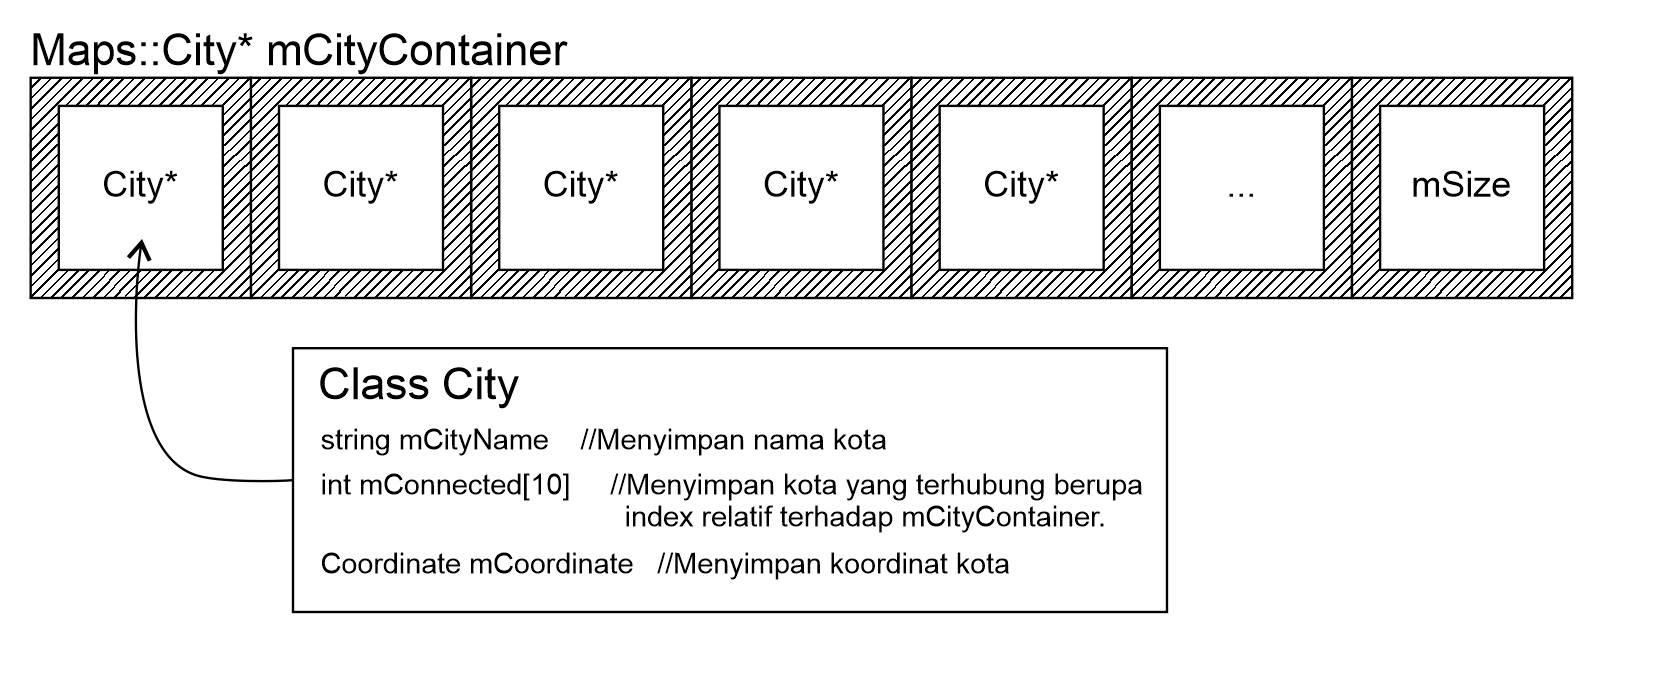
\includegraphics[width=12cm]{mCityContainer.png}
    \caption{Ilustrasi array mCityContainer}
    \label{fig:maps}
\end{figure}
\par
Dapat dilihat pada ilustrasi di atas, array ini menyimpan pointer dari objek City. Ukuran dari array ini sama dengan mSize yang mana mSize ditentukan pada saat melakukan kontruksi Class. Pada tiap-tiap class City
menyimpan mCityName (nama kota), mConnected dengan ukuran sebesar 10, dan coordinate. Pada mConnected disimpan index kota yang terhubung dengan kota bersangkutan. Index ini berdasarkan index kota yang ada pada array mCityContainer.
Alasan digunakannya index kota sebagai perefrensi kota yang terhubung adalah karena lebih efisien ketimbang menggunakan nama kota atau ID tetap terutama ketika ingin melakukan proses
path finding. Pada proses pathfinding biasanya dilakukan pemindaian tiap-tiap kota yang terkoneksi. Jika tidak menggunakan index, maka akan terjadi pencarian kota secara berulang kali. Hal ini tentunya akan memakan waktu. Meskipun begitu,
tentu terdapat hal yang perlu dikorbankan yaitu pada saat melakukan penghapusan dan penyisipan kota. Setiap kali melakukan kedua operasi tersebut maka perlu melakukan pengupdatean pada setiap kota yang ada. Tetapi hal ini bukan suatu masalah,
karena kedua operasi tersebut jarang dipakai dibandingkan dengan proses pathfinding yang lebih sering dipaakai.
\subsection{Class Queue}
\par
Class ini menerapkan prinsip FIFO. FIFO adalah suatu struktur data yang menyimpan data secara berurutan. FIFO dapat digunakan untuk menyimpan data yang berurutan. Penyimpanan objek pada class ini menggunakan array yang ukurannya ditentukan pada saat mengkontruksi class.
\begin{figure}[htp]
    \centering
    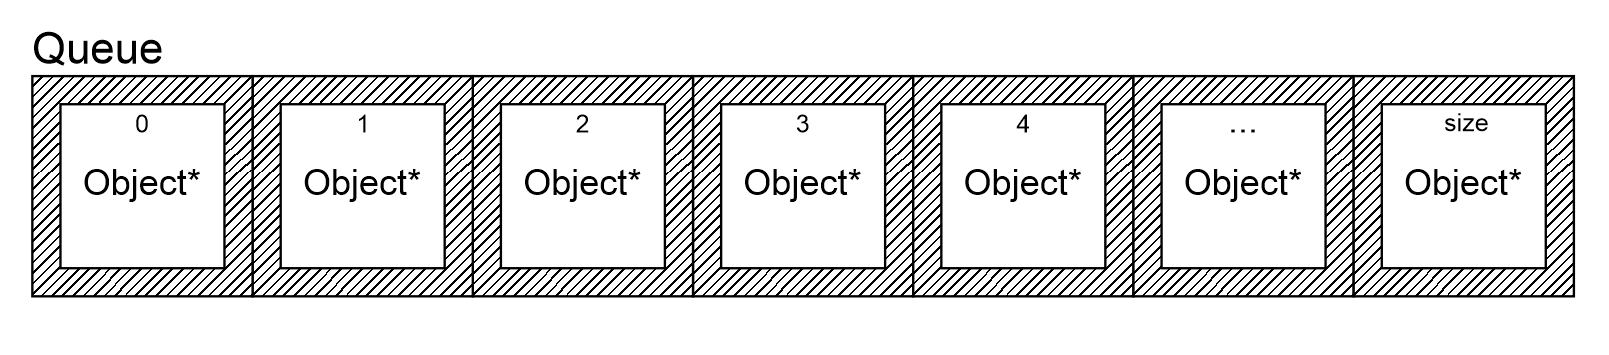
\includegraphics[width=12cm]{queue.png}
    \caption{Ilustrasi class Queue}
    \label{fig:queue}
\end{figure}
\subsection{Class Stack}
Berbeda dengan class Queue, class Stack menyimpan data dengan prinsip LIFO. Prinsip ini dapat diibaratkan sebagai tumpukan piring, dimana objek yang terakhir dimasukkan adalah objek yang pertama dikeluarkan. Karena Class stack dan queue sama-sama menggunakan array untuk menyimpan objeknya, ilustrasi dari class Stack dan Queue adalah sama.
Hal yang membedakan dari kedua class tersebut adalah operasi fungsinya yang akan dijelaskan pada bagian Penjelasan Program.
\begin{figure}[htp]
    \centering
    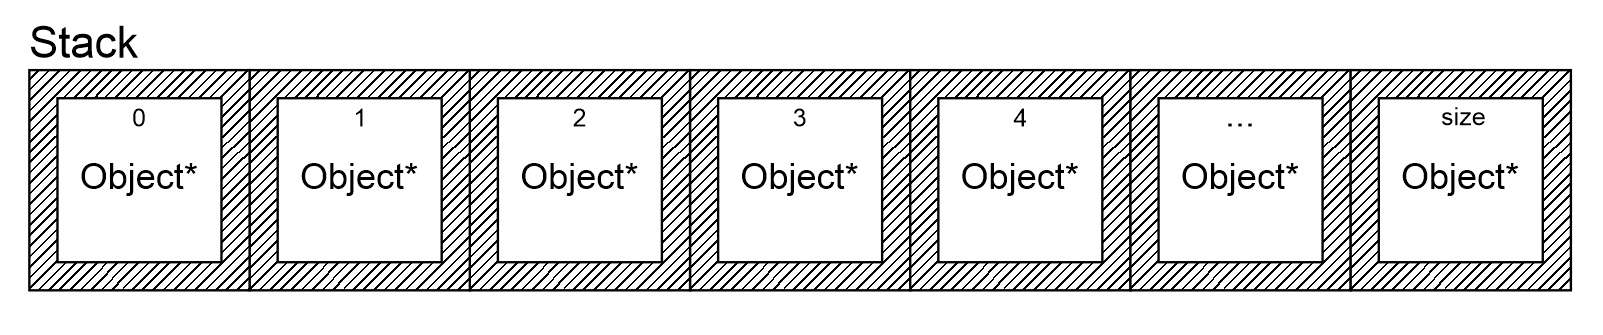
\includegraphics[width=12cm]{stack.png}
    \caption{Ilustrasi class Stack}
    \label{fig:stack}
\end{figure}
\pagebreak
\section{Penjelasan Program}
\par
Pada program ini digunakan library tambahan, yaitu SFML yang digunakan untuk memvisualisasikan hubungan kota. Seperti yang telah disebutkan pada bagian Desain Struktur Data,
pada program ini terdapat class Maps, City, CityPoint, dan Struct Coordinate.
\subsection{Class Maps}
Class ini berisikan method-method yang digunakan untuk mengatur kota seperti menambah (addCity()), menghapus (remove()), menyisipkan (insert()), mencari kota (findCityByName()) dan menghubungkan kota (connect()).
Penambahan kota dilakukan dengan cara:
\begin{enumerate}
    \item Membuat object City baru bernama newCity.
    \item Melakukan pengecekan ukuran Maps. Jika ukuran Maps masih cukup maka akan dilakukan penambahan kota.
    \item Pada akhir fungsi dilakukan pengembalian *this, sehingga fungsi ini dapat dipanggil kembali secara beruntun.
\end{enumerate}
Penghapusan kota dilakukan dengan cara:
\begin{enumerate}
    \item Melakukan pencarian index kota yang akan dihapus dengan menggunakan fungsi findCityByname.
    \item Memindahkan elemen sebelah kanan kota yang akan dihapus ke index kota yang akan dihapus. Proses ini dilakukan secara terus menerus sampai ujung array.
    \item Melakukan pengupdatean array mConnected yang terdapat pada setiap object City. Pengupdatean ini akan dijabarkan pada penjelasan di bawah.
    \item Mengurangi ukuran Maps.
\end{enumerate}
Menyisipkan kota dilakukan dengan cara:
\begin{enumerate}
    \item Membuat object City baru bernama newCity.
    \item Melakukan pengecekan ukuran Maps. Jika ukuran Maps masih cukup maka akan dilakukan penambahan kota.
    \item Melakukan pergeseran elemen n ke n+1, dimana n adalah elemen terakhir pada array mCityContainer. Setelah dilakukan pergeseran n mundur ke n-1. Proses ini dilakukan berulang kali sampai n = index yang akan disisipkan.
    \item Melakukan pengisian elemen pada index n dengan newCity.
    \item Melakukan pengupdatean array mConnected yang terdapat pada setiap object Node.
    \item Menambahkan ukuran Maps dengan menambah mCurrSize dengan 1.
\end{enumerate}
Mencari kota dilakukan dengan cara:
\begin{enumerate}
    \item Melakukan transversal pada array maps. Jika nama kota yang dicari sama dengan nama kota pada array maka akan dikembalikan index kota.
    \item Jika tidak ada kota yang sama maka akan dikembalikan nilai -1.
\end{enumerate}
Menghubungkan kota dilakukan dengan cara:
\begin{enumerate}
    \item Melakukan pencarian index kota yang akan dihubungkan dengan menggunakan fungsi findCityByname. Jika salah satu dari index bernilai -1 maka proses akan dibatalkan dengan melakukan return.
    \item Melakukan pemanggilan method Connect() yang terdapat pada Class City.
    \item Pada fungsi City::Connect() dilakukan transversal untuk mengecek apakah kota tersebut sudah terhubung atau belum. Jika belum maka dilakukan penambahan index kota yang akan dihubungkan ke array mConnected.
\end{enumerate}
\subsection{Class City}
\par
Class ini berfungsi untuk menyimpan informasi kota seperti nama, koordinat, dan jumlah kota yang terhubung. Selain menyimpan informasi kota,
pada class ini juga terdapat method-method yang digunakan untuk mengupdate index pada mConnected jika terjadi perubahan penomoran index pada mCityContainer.
\subsection{Struct Coordinate}
\par
Pada struct ini terdapat 2 member x dan y berupa int yang berfungsi untuk menyimpan koordinat kota. Terdapat juga Constructor agar memudahkan penginisasian koordinat. Selain itu, dibuat method
bernama formatedString dan operator overloading untuk operator \(<\!\!<\) agar memudahkan penulisan koordinat.
\subsection{CityPoint}
\par
Class ini digunakan dalam memvisualisakian hubungan kota. Class ini merupakan turunan dari Class Drawable yang terdapat pada library SFML. 
Pada class ini dilakukan pembuatan shape berbentuk lingkaran, text nama kota, dan text koordinat kota. Dari ketiga objek tersebut ditata sedemikian rupa.
\subsection{Stack}
Class ini merupakan implementasi dari data stuktur stack. 
Agar tidak perlu melakukan perulangan penulisan pada setiap data type digunakanlah fitur template. 
Untuk penyimpan objek pada class ini menggunakan array. 
Terdapat method-method dasar stack seperti push(), pop(), top(), dan empty(). 
Di bawah ini merupakan ilustrasi dari method-method tersebut.
\begin{figure}[H]
    \centering
    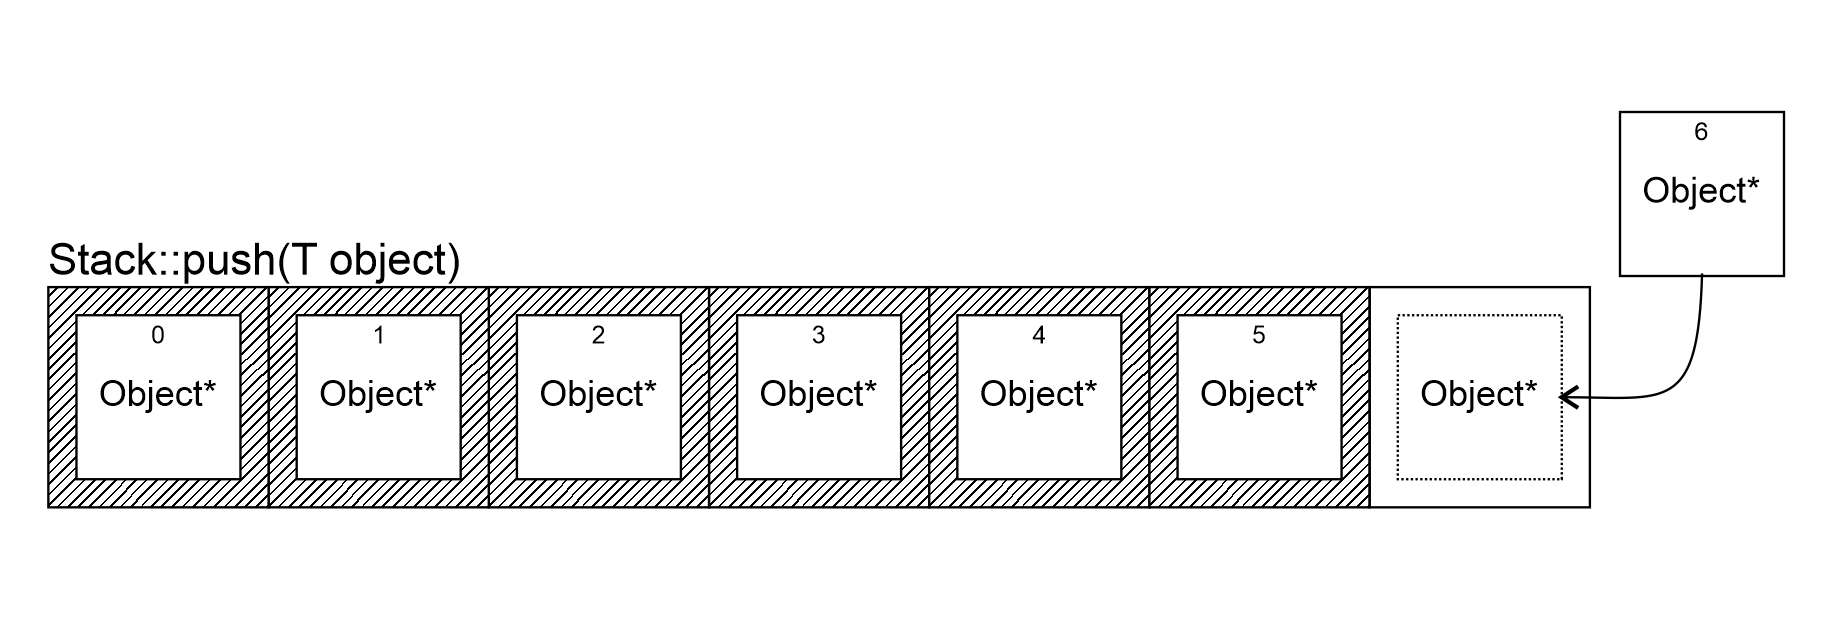
\includegraphics[width=12cm]{stackpush.png}
    \caption{Ilustrasi method Stack::push()}
    \label{fig:stackpush}
\end{figure}
Terlihat seperti pada ilustrasi di atas, objek yang dimasukkan akan disimpan di index terakhir pada array.
\begin{figure}[H]
    \centering
    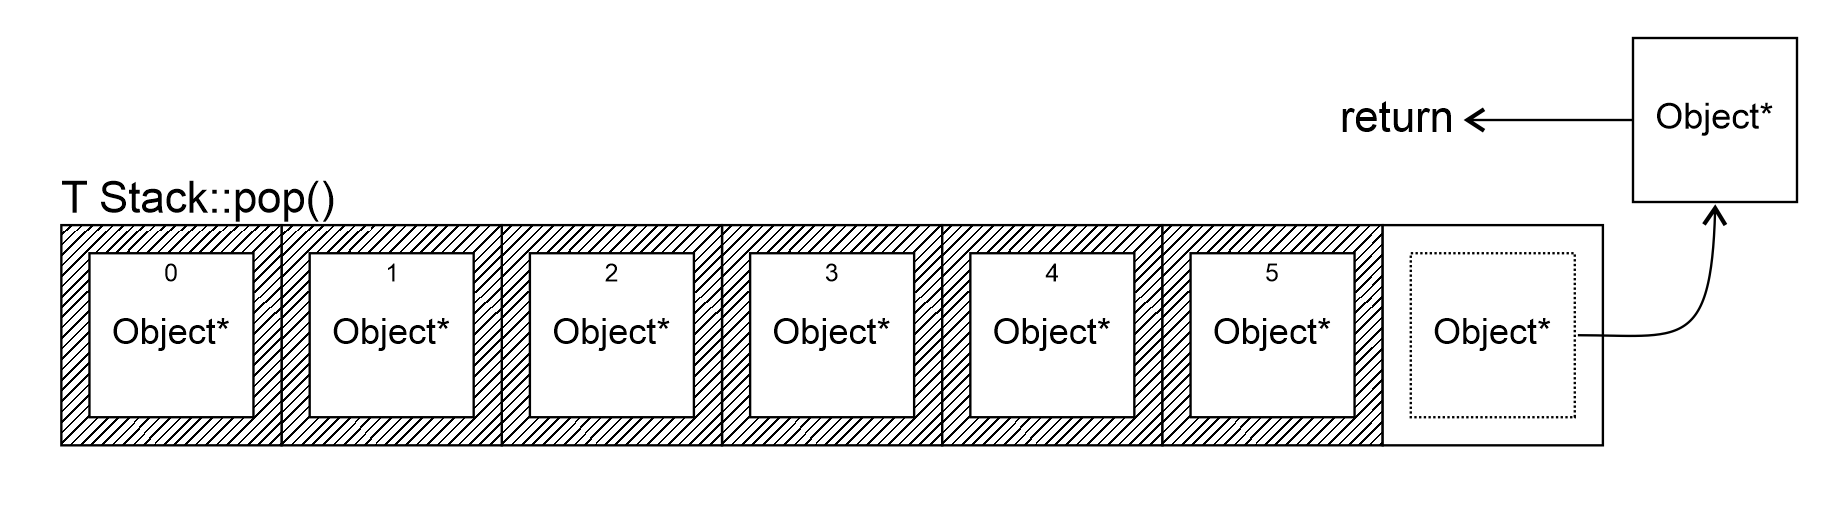
\includegraphics[width=12cm]{stackpop.png}
    \caption{Ilustrasi method Stack::pop()}
    \label{fig:stackpop}
\end{figure}
Pada method pop akan dilakukan return objek yang terakhir dimasukkan sekaligus menghapusnya dari array.
\begin{figure}[H]
    \centering
    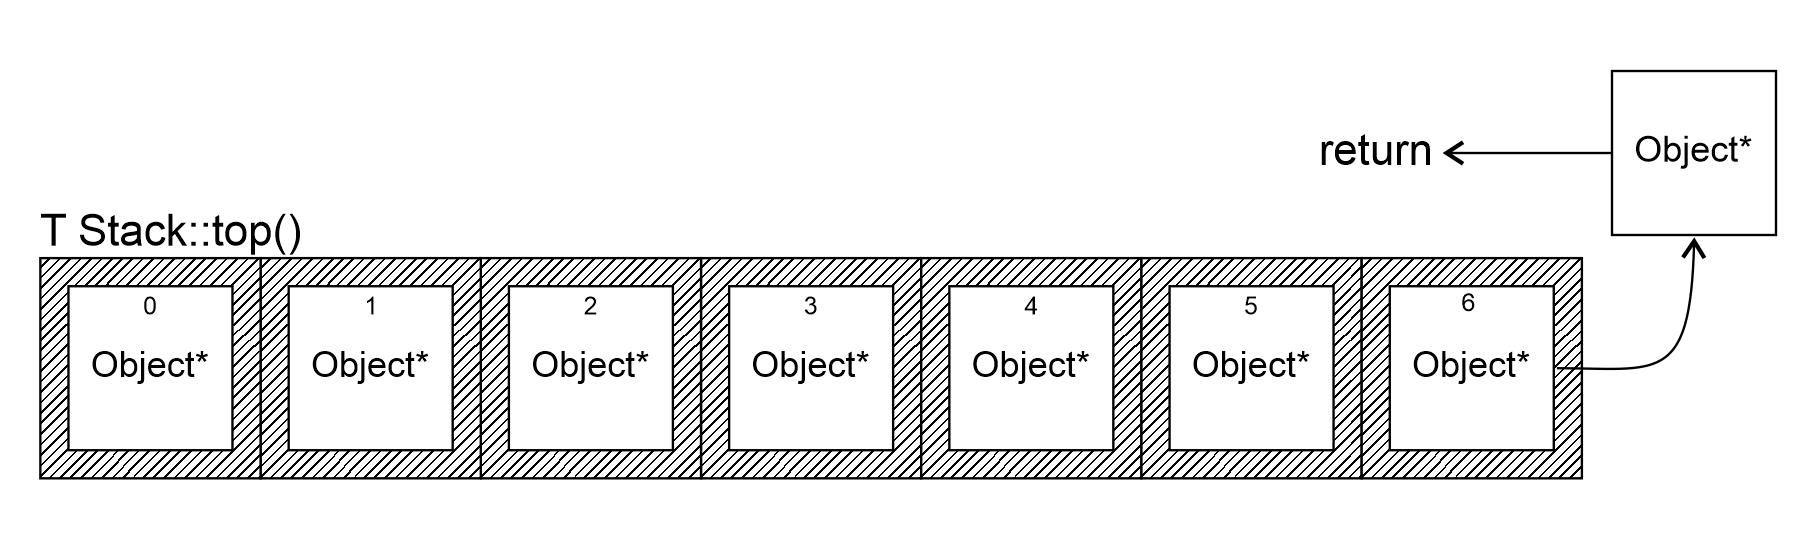
\includegraphics[width=12cm]{stacktop.png}
    \caption{Ilustrasi method Stack::top()}
    \label{fig:stacktop}
\end{figure}
Sama dengan method pop hanya saja pada method ini tidak dilakukan penghapusan objek.
\subsection{Queue}
\par
Class ini merupakan implementasi dari data stuktur queue. Sama halnya dengan class Stack, class ini menggunakan array unutk menyimpan objeknya dan memanfaatkan fitur template agar tidak perlu melakukan perulangan penulisan pada setiap data type.
Method-method yang terdapat pada class ini didasarkan pada method dasar queue yang ada pada bahasa python seperti get(), put(), dan empty(). Di bawah ini merupakan ilustrasi dari method get() dan put() yang terdapat pada class Queue.
\begin{figure}[htp]
    \centering
    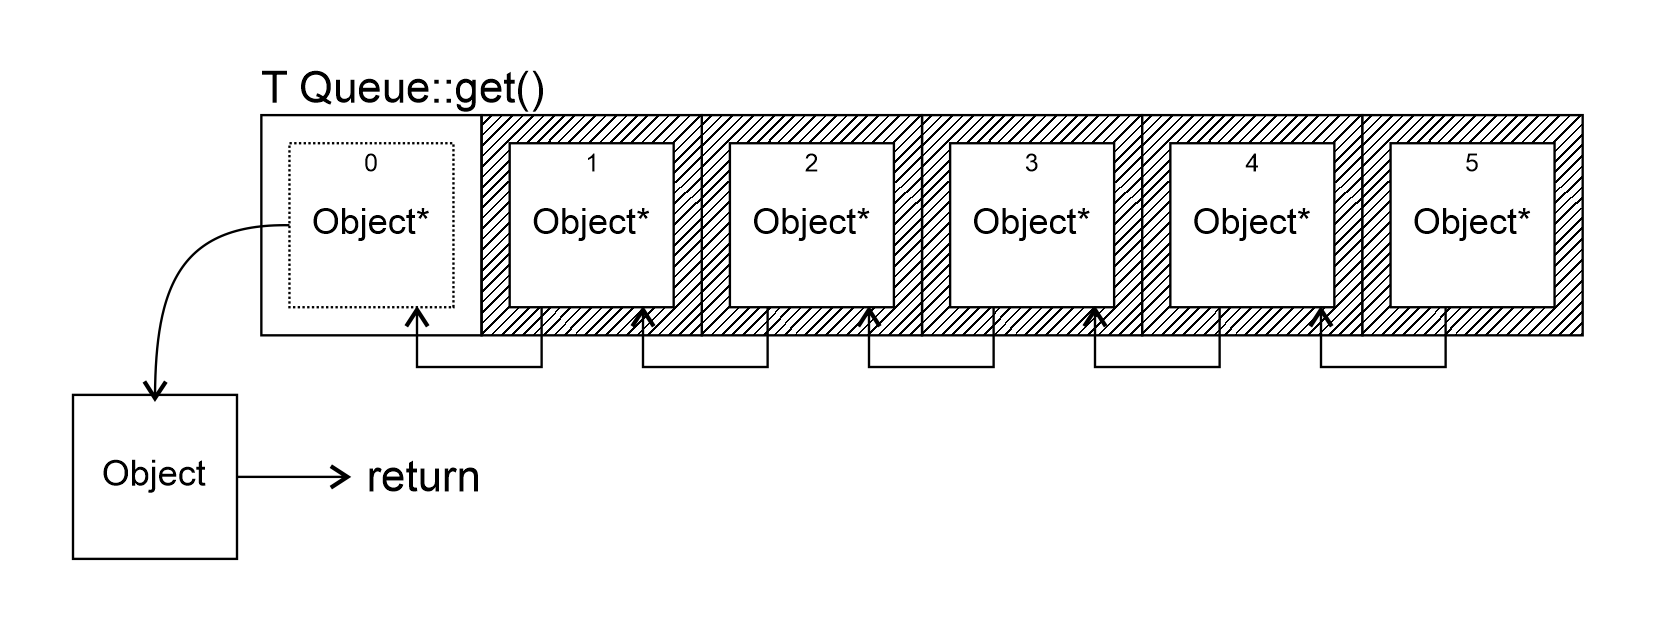
\includegraphics[width=12cm]{queueget.png}
    \caption{Ilustrasi method Queue::get()}
    \label{fig:queueget}
\end{figure}
\par
Terlihat pada ilustrasi di atas bahwa method ini akan mereturn objek yang pertama dimasukkan sekaligus menghapusnya. Setelah dilakukan penghapusan maka objek yang berada di sebelahnya akan dipindah untuk mengisi kekosongan.
\begin{figure}[htp]
    \centering
    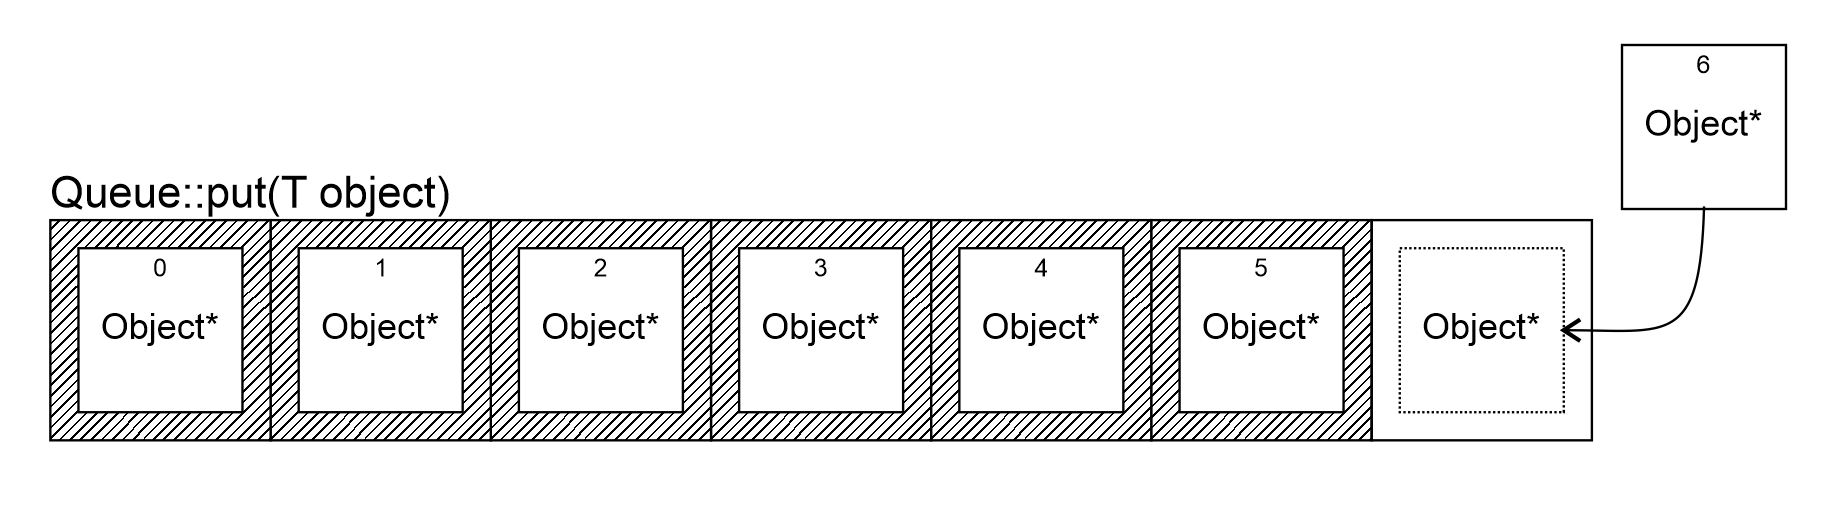
\includegraphics[width=12cm]{queueput.png}
    \caption{Ilustrasi method Queue::put()}
    \label{fig:queueput}
\end{figure}
\par
Penambahan objek dengan pemanggilan method put() dilakukan dengan menaruh objek yang akan dimasukkan kedalam array pada index terakhir.
\subsection{Fungsi Maps::visualize()}
\par
Fungsi ini terdapat pada class Maps. Fungsi ini digunakan untuk memvisualisasikan hubungan kota. Di bawah ini merupakan penjelasan dari fungsi ini.
\lstinputlisting[label={kodingan},caption={Fungsi visualize()}, language={C++}, firstline=284, lastline=372]{ets.cpp}
\begin{enumerate}
    \item Line 3-8: Melakukan penginisasian objek window, font, dan container objek CityPoint.
    \item Line 12-16: Melakukan transversal pada seluruh mCityContainer. Setiap kota yang ditemukan maka akan dicreate menjadi CityPoint. Penempatan objek CityPoint didsarkan pada koordinat kota.
    \item Line 18-27: Melakukan tranversal pada array mConnected yang terdapat pada objek City. Jika objek City tersebut terhubung dengan kota lain maka akan dilakukan pemanggilan method connect() yang terdapat pada class CityPoint. Dengan pemanggilan ini maka akan terbentuk garis yang menghubungkan kedua kota tersebut.
    \item Line 29-79: Baris ini befungsi untuk menghandle control dari mouse seperti zoom dan drag to move.
    \item Line 81-87: Baris ini berfungsi untuk menampilkan objek CityPoint ke layar.
\end{enumerate}
\end{document}
